% ============================================================
%  Semaine 2 — HTML5 : structure & sémantique
%  PRÉSENTATION (Beamer) — cfpt·i | Anne Terrier
%  Charte graphique : cfpt·i (bleu accentBlue + jaune cfptYellow)
% ============================================================
\documentclass[aspectratio=169,11pt]{beamer}

\usepackage[T1]{fontenc}
\usepackage[utf8]{inputenc}
\usepackage[scaled=0.92]{helvet}
\renewcommand{\familydefault}{\sfdefault}

\usepackage{tikz}
\usetikzlibrary{positioning, arrows.meta, decorations.pathreplacing}
\usepackage{booktabs}
\usepackage{tabularx}
\usepackage{colortbl}
\usepackage{listings}

% ---------------------------------------------------------------
% Palette cfpt·i
% ---------------------------------------------------------------
\definecolor{cfptYellow}{HTML}{F5C400}
\definecolor{cfptBlack}{HTML}{1A1A1A}
\definecolor{cfptDarkGrey}{HTML}{555555}
\definecolor{cfptGrey}{HTML}{F2F2F2}
\definecolor{accentBlue}{HTML}{1D4E89}
\definecolor{lightBlue}{HTML}{D6E4F0}
\definecolor{codeGrey}{HTML}{F5F5F5}
\definecolor{successGreen}{HTML}{1E7145}
\definecolor{warningOrange}{HTML}{C55A11}

% Alias (repris du polycop)
\colorlet{uniInk}{cfptBlack}
\colorlet{uniNavy}{accentBlue}
\colorlet{uniTeal}{successGreen}
\colorlet{uniGold}{warningOrange}
\colorlet{uniGrey}{cfptDarkGrey}
\colorlet{uniPaper}{cfptGrey}
\colorlet{uniRule}{cfptDarkGrey!35}

% ---------------------------------------------------------------
% Thème Beamer personnalisé cfpt·i
% ---------------------------------------------------------------
\usetheme{default}
\usecolortheme{default}
\setbeamercolor{palette primary}{bg=accentBlue, fg=white}
\setbeamercolor{structure}{fg=accentBlue}
\setbeamercolor{frametitle}{bg=accentBlue, fg=white}
\setbeamercolor{title}{fg=white}
\setbeamercolor{block title}{bg=accentBlue, fg=white}
\setbeamercolor{block body}{bg=lightBlue!30, fg=cfptBlack}
\setbeamercolor{block title alerted}{bg=cfptYellow!85!black, fg=cfptBlack}
\setbeamercolor{block body alerted}{bg=cfptYellow!20, fg=cfptBlack}
\setbeamercolor{block title example}{bg=successGreen, fg=white}
\setbeamercolor{block body example}{bg=successGreen!8, fg=cfptBlack}
\setbeamercolor{itemize item}{fg=cfptYellow!85!black}
\setbeamercolor{itemize subitem}{fg=cfptDarkGrey}
\setbeamercolor{enumerate item}{fg=accentBlue}
\setbeamercolor{normal text}{fg=cfptBlack}
\setbeamercolor{footline}{fg=white}

\setbeamertemplate{itemize item}{\textbullet}
\setbeamertemplate{itemize subitem}{--}
\setbeamertemplate{navigation symbols}{}
\setbeamertemplate{blocks}[rounded][shadow=false]

% Titre de frame : bandeau plein largeur
\setbeamertemplate{frametitle}{%
  \nointerlineskip%
  \begin{beamercolorbox}[wd=\paperwidth, ht=2.6ex, dp=1.2ex, leftskip=0.3cm]{frametitle}%
    \usebeamerfont{frametitle}\bfseries\insertframetitle%
  \end{beamercolorbox}%
}

% Pied de page : logo texte + section + numéro
\setbeamertemplate{footline}{%
  \leavevmode%
  \hbox{%
    \begin{beamercolorbox}[wd=.32\paperwidth, ht=2.4ex, dp=1ex, leftskip=0.3cm]{palette primary}%
      \usebeamerfont{author in head/foot}\tiny Anne Terrier%
    \end{beamercolorbox}%
    \begin{beamercolorbox}[wd=.44\paperwidth, ht=2.4ex, dp=1ex, center]{palette primary}%
      \usebeamerfont{title in head/foot}\tiny Semaine 2 --- HTML5 : structure \& sémantique%
    \end{beamercolorbox}%
    \begin{beamercolorbox}[wd=.24\paperwidth, ht=2.4ex, dp=1ex, right, rightskip=0.3cm]{palette primary}%
      \usebeamerfont{date in head/foot}\tiny\insertframenumber\,/\,\inserttotalframenumber%
    \end{beamercolorbox}%
  }%
}

% ---------------------------------------------------------------
% Listings — coloration HTML
% ---------------------------------------------------------------
\lstset{
  basicstyle=\ttfamily\scriptsize,
  backgroundcolor=\color{codeGrey},
  frame=single, framerule=0.4pt,
  rulecolor=\color{cfptDarkGrey!40},
  breaklines=true,
  keywordstyle=\color{accentBlue}\bfseries,
  commentstyle=\color{cfptDarkGrey}\itshape,
  stringstyle=\color{successGreen},
  showstringspaces=false,
}

\lstdefinelanguage{HTML5}{
  keywords={<!DOCTYPE, html, head, body, header, nav, main, section, article, aside, footer, h1, h2, h3, p, a, img, ul, ol, li, table, thead, tbody, tr, th, td, form, input, textarea, select, option, label, button, div, span, meta, title, link, script},
  sensitive=false,
  morecomment=[s]{<!--}{-->},
  morestring=[b]",
  keywordstyle=\color{accentBlue}\bfseries,
  stringstyle=\color{warningOrange},
  commentstyle=\color{cfptDarkGrey}\itshape,
}

% ---------------------------------------------------------------
% Métadonnées
% ---------------------------------------------------------------
\title{HTML5 --- Structure \& sémantique}
\subtitle{Développement web --- Classe passerelle}
\author{Anne Terrier}
\institute{cfpt\textperiodcentered i --- École d'informatique}
\date{Semaine 2}

% ===============================================================
\begin{document}
% ===============================================================

% --- Diapo de titre ---
{
\setbeamertemplate{footline}{}
\begin{frame}[plain]
  \begin{tikzpicture}[remember picture, overlay]
    \fill[accentBlue] (current page.north west) rectangle ([yshift=-3.2cm]current page.north east);
    \node[anchor=north west, text=white, font=\huge\bfseries, text width=0.9\paperwidth]
      at ([shift={(0.8cm,-0.8cm)}]current page.north west)
      {HTML5 --- Structure \& sémantique};
    \node[anchor=north west, text=lightBlue, font=\large]
      at ([shift={(0.85cm,-2.55cm)}]current page.north west)
      {Développement web --- Classe passerelle};

    % accent jaune
    \fill[cfptYellow] ([yshift=-3.2cm]current page.north west) rectangle ([yshift=-3.35cm]current page.north east);

    \node[anchor=south west, font=\large\bfseries, text=accentBlue]
      at ([shift={(0.8cm,1.8cm)}]current page.south west) {Semaine 2};
    \node[anchor=south west, font=\normalsize, text=cfptDarkGrey]
      at ([shift={(0.8cm,1.1cm)}]current page.south west)
      {Anne Terrier \quad\textbar\quad cfpt\textperiodcentered i --- École d'informatique};
  \end{tikzpicture}
\end{frame}
}

% --- Plan ---
\begin{frame}{Au programme aujourd'hui}
  \begin{columns}[T]
    \begin{column}{0.48\textwidth}
      \begin{enumerate}
        \item Qu'est-ce que le HTML ?
        \item La structure d'un document
        \item Les éléments sémantiques
        \item Texte, liens \& images
      \end{enumerate}
    \end{column}
    \begin{column}{0.48\textwidth}
      \begin{enumerate}
        \setcounter{enumi}{4}
        \item Listes \& tableaux
        \item Les formulaires
        \item Accessibilité
      \end{enumerate}
      \vspace{0.5cm}
      \begin{block}{Objectif de la semaine}
        Écrire une page HTML5 valide et sémantique, et construire un premier formulaire.
      \end{block}
    \end{column}
  \end{columns}
\end{frame}

% ===============================================================
\section{Qu'est-ce que le HTML ?}
% ===============================================================
{
\setbeamertemplate{footline}{}
\begin{frame}[plain]
  \begin{tikzpicture}[remember picture, overlay]
    \fill[accentBlue] (current page.north west) rectangle (current page.south east);
    \fill[cfptYellow] ([yshift=-0.15cm]current page.center -| current page.west)
      rectangle ([yshift=-0.3cm]current page.center -| current page.east);
    \node[text=white, font=\Huge\bfseries] at ([yshift=0.9cm]current page.center)
      {1. Qu'est-ce que le HTML ?};
  \end{tikzpicture}
\end{frame}
}

\begin{frame}{Un langage de balisage}
  \begin{block}{Définition}
    Le HTML (\textit{HyperText Markup Language}) décrit la \textbf{structure} et le \textbf{contenu} d'une page web.
  \end{block}
  \vspace{0.3cm}
  \begin{alertblock}{Ce n'est pas un langage de programmation}
    On ne « programme » pas en HTML : on \textbf{balise} le contenu pour indiquer au navigateur ce que chaque morceau représente --- un titre, un paragraphe, une image, un lien\dots
  \end{alertblock}
  \vspace{0.3cm}
  \begin{center}
    \small Pour créer une page web : un simple fichier avec l'extension \textbf{.html}.
  \end{center}
\end{frame}

\begin{frame}{Anatomie d'une balise}
  \vspace{0.5cm}
  \begin{center}
  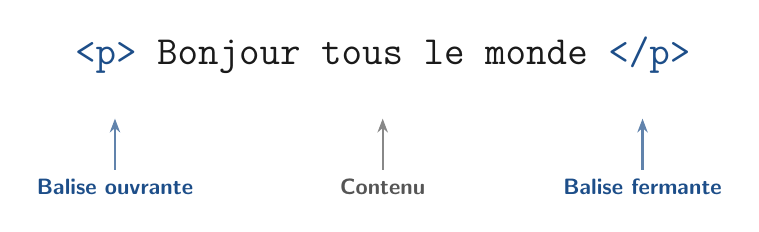
\begin{tikzpicture}[font=\small]
    \node[font=\ttfamily\Large] (code) {%
      \textcolor{accentBlue}{<p>}%
      \textcolor{cfptBlack}{~Bonjour tous le monde~}%
      \textcolor{accentBlue}{</p>}};
    \node[below=1.1cm of code, xshift=-3.4cm, text=accentBlue, font=\footnotesize\bfseries] (lo) {Balise ouvrante};
    \node[below=1.1cm of code, xshift=0cm, text=cfptDarkGrey, font=\footnotesize\bfseries] (ct) {Contenu};
    \node[below=1.1cm of code, xshift=3.3cm, text=accentBlue, font=\footnotesize\bfseries] (lf) {Balise fermante};
    \draw[-{Stealth[length=5pt]}, accentBlue!70, thick] (lo.north) -- ++(0,0.65);
    \draw[-{Stealth[length=5pt]}, cfptDarkGrey!70, thick] (ct.north) -- ++(0,0.65);
    \draw[-{Stealth[length=5pt]}, accentBlue!70, thick] (lf.north) -- ++(0,0.65);
  \end{tikzpicture}
  \end{center}
  \vspace{0.4cm}
  \begin{exampleblock}{Balises auto-fermantes}
    Certaines balises n'encadrent aucun contenu et s'écrivent seules : \texttt{<img>} (image), \texttt{<br>} (retour à la ligne).
  \end{exampleblock}
\end{frame}

\begin{frame}[fragile]{Les attributs}
  Une balise peut porter des \textbf{attributs}, qui précisent son comportement, sous la forme \texttt{nom="valeur"} :
  \vspace{0.3cm}
\begin{lstlisting}[language=HTML5]
<a href="https://www.hepia.ch">Site de la hepia</a>
\end{lstlisting}
  \vspace{0.3cm}
  \begin{center}
    \small Ici, \texttt{href} est l'attribut qui indique la \textbf{destination} du lien.
  \end{center}
\end{frame}

% ===============================================================
\section{La structure d'un document HTML5}
% ===============================================================
{
\setbeamertemplate{footline}{}
\begin{frame}[plain]
  \begin{tikzpicture}[remember picture, overlay]
    \fill[accentBlue] (current page.north west) rectangle (current page.south east);
    \fill[cfptYellow] ([yshift=-0.15cm]current page.center -| current page.west)
      rectangle ([yshift=-0.3cm]current page.center -| current page.east);
    \node[text=white, font=\Huge\bfseries] at ([yshift=0.9cm]current page.center)
      {2. La structure d'un document};
  \end{tikzpicture}
\end{frame}
}

\begin{frame}[fragile]{Le squelette d'une page HTML5}
\begin{lstlisting}[language=HTML5]
<!DOCTYPE html>
<html lang="fr">
<head>
  <meta charset="UTF-8">
  <title>Titre de la page</title>
</head>
<body>
  <!-- Le contenu visible va ici -->
</body>
</html>
\end{lstlisting}
  \begin{alertblock}{À retenir --- head vs body}
    Le \texttt{<head>} contient des informations \emph{sur} la page (titre, encodage). Le \texttt{<body>} contient tout le contenu \textbf{visible}.
  \end{alertblock}
\end{frame}

% ===============================================================
\section{Les éléments sémantiques}
% ===============================================================
{
\setbeamertemplate{footline}{}
\begin{frame}[plain]
  \begin{tikzpicture}[remember picture, overlay]
    \fill[accentBlue] (current page.north west) rectangle (current page.south east);
    \fill[cfptYellow] ([yshift=-0.15cm]current page.center -| current page.west)
      rectangle ([yshift=-0.3cm]current page.center -| current page.east);
    \node[text=white, font=\Huge\bfseries] at ([yshift=0.9cm]current page.center)
      {3. Les éléments sémantiques};
  \end{tikzpicture}
\end{frame}
}

\begin{frame}{Décrire le rôle de chaque zone}
  \begin{center}
  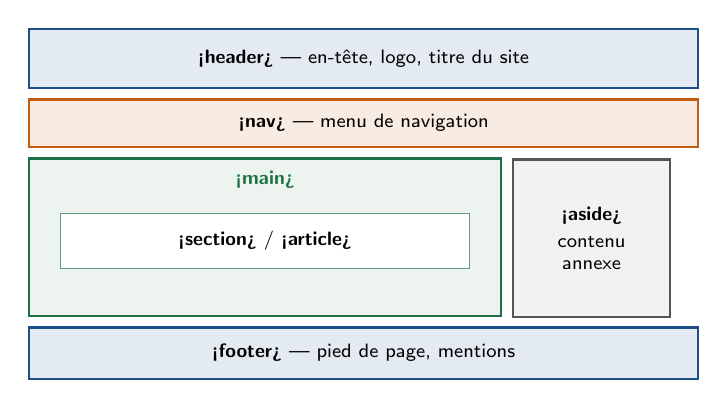
\begin{tikzpicture}[font=\scriptsize, every node/.style={align=center}]
    \node[draw=accentBlue, fill=accentBlue!12, thick, minimum width=8.5cm, minimum height=0.75cm] (header) {\textbf{<header>} --- en-tête, logo, titre du site};
    \node[draw=warningOrange, fill=warningOrange!12, thick, minimum width=8.5cm, minimum height=0.6cm, below=0.12cm of header] (nav) {\textbf{<nav>} --- menu de navigation};
    \node[draw=successGreen, fill=successGreen!8, thick, minimum width=6cm, minimum height=2cm, below=0.12cm of nav, xshift=-1.25cm, anchor=north] (main) {};
    \node[text=successGreen, font=\scriptsize\bfseries] at ([yshift=-0.28cm]main.north) {<main>};
    \node[draw=successGreen!70, fill=white, minimum width=5.2cm, minimum height=0.7cm] at ([yshift=-0.05cm]main.center) {\textbf{<section>} / \textbf{<article>}};
    \node[draw=cfptDarkGrey, fill=cfptGrey, thick, minimum width=2cm, minimum height=2cm, right=0.12cm of main, anchor=north west, yshift=1.0cm] (aside) {\textbf{<aside>}\\[2pt]\scriptsize contenu\\annexe};
    \node[draw=accentBlue, fill=accentBlue!12, thick, minimum width=8.5cm, minimum height=0.65cm, below=0.12cm of main, xshift=1.25cm] (footer) {\textbf{<footer>} --- pied de page, mentions};
  \end{tikzpicture}
  \end{center}
  \vspace{0.2cm}
  \begin{exampleblock}{Section ou article ?}
    Un \texttt{<article>} a du sens \textbf{tout seul} (un message de forum citable ailleurs). Une \texttt{<section>} regroupe des contenus liés par un \textbf{thème}.
  \end{exampleblock}
\end{frame}

\begin{frame}{Pourquoi la sémantique ?}
  Avant HTML5, les pages n'étaient que des \texttt{<div>} empilées. Les balises sémantiques rendent le code plus clair pour :
  \vspace{0.3cm}
  \begin{itemize}
    \item les \textbf{développeurs} qui relisent le code
    \item les \textbf{moteurs de recherche} (référencement)
    \item les \textbf{outils d'accessibilité} (lecteurs d'écran)
  \end{itemize}
  \vspace{0.4cm}
  \begin{block}{Le réflexe}
    Choisir sa balise selon le \textbf{sens} du contenu, jamais selon son apparence. L'apparence, ce sera le rôle du CSS (semaine 3).
  \end{block}
\end{frame}

% ===============================================================
\section{Texte, liens \& images}
% ===============================================================
{
\setbeamertemplate{footline}{}
\begin{frame}[plain]
  \begin{tikzpicture}[remember picture, overlay]
    \fill[accentBlue] (current page.north west) rectangle (current page.south east);
    \fill[cfptYellow] ([yshift=-0.15cm]current page.center -| current page.west)
      rectangle ([yshift=-0.3cm]current page.center -| current page.east);
    \node[text=white, font=\Huge\bfseries] at ([yshift=0.9cm]current page.center)
      {4. Texte, liens \& images};
  \end{tikzpicture}
\end{frame}
}

\begin{frame}[fragile]{Titres, liens et images}
\begin{lstlisting}[language=HTML5]
<h1>Titre principal (un seul par page)</h1>
<h2>Sous-titre</h2>
<p>Un paragraphe avec du <strong>texte important</strong>.</p>

<a href="contact.html">Nous contacter</a>

<img src="logo.png" alt="Logo du MiniForum">
\end{lstlisting}
  \begin{alertblock}{Deux règles à ne pas oublier}
    Un seul \texttt{<h1>} par page, sans sauter de niveau de titre. Et toujours un attribut \texttt{alt} sur les images.
  \end{alertblock}
\end{frame}

\begin{frame}[fragile]{L'attribut \texttt{id} : identifier un élément}
  Un \texttt{id} donne un \textbf{nom unique} à un élément. On peut ensuite pointer vers lui :
\begin{lstlisting}[language=HTML5]
<a href="#contact">Aller au formulaire</a>

<section id="contact"> ... </section>
\end{lstlisting}
  \vspace{0.1cm}
  \begin{columns}[T]
    \begin{column}{0.5\textwidth}
      \begin{alertblock}{Règle d'or}
        Un \texttt{id} est \textbf{unique} dans la page : jamais deux fois le même.
      \end{alertblock}
    \end{column}
    \begin{column}{0.5\textwidth}
      \begin{block}{Un point d'accroche}
        Réutilisé partout : \texttt{label}, \textbf{CSS} (sem. 3), \textbf{JS} (\texttt{getElementById}).
      \end{block}
    \end{column}
  \end{columns}
\end{frame}

% ===============================================================
\section{Listes \& tableaux}
% ===============================================================
{
\setbeamertemplate{footline}{}
\begin{frame}[plain]
  \begin{tikzpicture}[remember picture, overlay]
    \fill[accentBlue] (current page.north west) rectangle (current page.south east);
    \fill[cfptYellow] ([yshift=-0.15cm]current page.center -| current page.west)
      rectangle ([yshift=-0.3cm]current page.center -| current page.east);
    \node[text=white, font=\Huge\bfseries] at ([yshift=0.9cm]current page.center)
      {5. Listes \& tableaux};
  \end{tikzpicture}
\end{frame}
}

\begin{frame}[fragile]{Listes ordonnées et non ordonnées}
  \begin{columns}[T]
    \begin{column}{0.5\textwidth}
      \begin{center}\footnotesize\textbf{Liste à puces}\end{center}
\begin{lstlisting}[language=HTML5]
<ul>
  <li>HTML</li>
  <li>CSS</li>
  <li>JavaScript</li>
</ul>
\end{lstlisting}
    \end{column}
    \begin{column}{0.5\textwidth}
      \begin{center}\footnotesize\textbf{Liste numérotée}\end{center}
\begin{lstlisting}[language=HTML5]
<ol>
  <li>Ouvrir le terminal</li>
  <li>Taper la commande</li>
  <li>Valider</li>
</ol>
\end{lstlisting}
    \end{column}
  \end{columns}
  \vspace{0.3cm}
  \begin{center}
    \small \texttt{<ol>} quand l'ordre compte, \texttt{<ul>} quand il est indifférent.
  \end{center}
\end{frame}

\begin{frame}[fragile]{Les tableaux}
\begin{lstlisting}[language=HTML5]
<table>
  <thead>
    <tr><th>Sujet</th><th>Auteur</th></tr>
  </thead>
  <tbody>
    <tr><td>Bienvenue</td><td>Alice</td></tr>
  </tbody>
</table>
\end{lstlisting}
  \begin{alertblock}{Attention}
    Un tableau sert à présenter des \textbf{données}, jamais à mettre en page une interface --- ça, c'est le rôle du CSS.
  \end{alertblock}
\end{frame}

% ===============================================================
\section{Les formulaires}
% ===============================================================
{
\setbeamertemplate{footline}{}
\begin{frame}[plain]
  \begin{tikzpicture}[remember picture, overlay]
    \fill[accentBlue] (current page.north west) rectangle (current page.south east);
    \fill[cfptYellow] ([yshift=-0.15cm]current page.center -| current page.west)
      rectangle ([yshift=-0.3cm]current page.center -| current page.east);
    \node[text=white, font=\Huge\bfseries] at ([yshift=0.9cm]current page.center)
      {6. Les formulaires};
  \end{tikzpicture}
\end{frame}
}

\begin{frame}{Le champ \texttt{<input>} et ses types}
  La balise \texttt{<input>} change de comportement selon son attribut \texttt{type} :
  \vspace{0.2cm}
  \begin{center}
  \renewcommand{\arraystretch}{1.2}
    \begin{tabularx}{\linewidth}{p{3.2cm}X}
    \toprule
    \rowcolor{accentBlue}
    \color{white}\textbf{type} & \color{white}\textbf{Usage} \\
    \midrule
    \rowcolor{cfptGrey}
    \texttt{text} & Texte libre sur une ligne \\
    \texttt{email} & Adresse e-mail (validée automatiquement) \\
    \rowcolor{cfptGrey}
    \texttt{password} & Mot de passe (caractères masqués) \\
    \texttt{number} & Valeur numérique \\
    \rowcolor{cfptGrey}
    \texttt{checkbox} / \texttt{radio} & Case à cocher / choix unique \\
    \bottomrule
  \end{tabularx}
  \end{center}
\end{frame}

\begin{frame}[fragile]{Un formulaire complet}
\begin{lstlisting}[language=HTML5]
<form>
  <label for="pseudo">Votre pseudo :</label>
  <input type="text" id="pseudo" name="pseudo">

  <label for="message">Votre message :</label>
  <textarea id="message" name="message"></textarea>

  <button type="submit">Envoyer</button>
</form>
\end{lstlisting}
  \begin{alertblock}{Le lien label / input}
    L'attribut \texttt{for} du \texttt{<label>} doit correspondre à l'\texttt{id} de l'\texttt{<input>}. Indispensable pour l'accessibilité.
  \end{alertblock}
\end{frame}

% ===============================================================
\section{Accessibilité}
% ===============================================================
{
\setbeamertemplate{footline}{}
\begin{frame}[plain]
  \begin{tikzpicture}[remember picture, overlay]
    \fill[accentBlue] (current page.north west) rectangle (current page.south east);
    \fill[cfptYellow] ([yshift=-0.15cm]current page.center -| current page.west)
      rectangle ([yshift=-0.3cm]current page.center -| current page.east);
    \node[text=white, font=\Huge\bfseries] at ([yshift=0.9cm]current page.center)
      {7. Accessibilité};
  \end{tikzpicture}
\end{frame}
}

\begin{frame}{Les bons réflexes dès le HTML}
  Rendre la page utilisable par tous, y compris les personnes en situation de handicap :
  \vspace{0.3cm}
  \begin{itemize}
    \item Toujours renseigner l'attribut \texttt{alt} des images
    \item Respecter la hiérarchie des titres (\texttt{<h1>} puis \texttt{<h2>}\dots)
    \item Associer chaque \texttt{<input>} à un \texttt{<label>}
    \item Préférer les balises sémantiques aux \texttt{<div>}
    \item Préciser la langue : \texttt{<html lang="fr">}
  \end{itemize}
  \vspace{0.3cm}
  \begin{block}{Valider son code}
    Le service \textbf{validator.w3.org} vérifie qu'une page est correctement écrite. Un HTML valide est la base d'un site fiable.
  \end{block}
\end{frame}

% ===============================================================
% Exercice intermédiaire
% ===============================================================
{
\setbeamertemplate{footline}{}
\begin{frame}[plain]
  \begin{tikzpicture}[remember picture, overlay]
    \fill[successGreen] (current page.north west) rectangle (current page.south east);
    \fill[cfptYellow] ([yshift=-0.15cm]current page.center -| current page.west)
      rectangle ([yshift=-0.3cm]current page.center -| current page.east);
    \node[text=white, font=\Huge\bfseries] at ([yshift=1.4cm]current page.center)
      {\raisebox{-2pt}{$\blacktriangleright$}~~À vous de jouer !};
    \node[text=white, font=\large, text width=0.8\paperwidth, align=center]
      at ([yshift=-0.6cm]current page.center)
      {Exercice intermédiaire --- Votre première page HTML};
  \end{tikzpicture}
\end{frame}
}

\begin{frame}{Exercice intermédiaire --- Votre première page HTML}
  \begin{exampleblock}{Objectif}
    Créer, seul·e, une page \texttt{index.html} valide et sémantique, avant d'attaquer le squelette du MiniForum en TP.
  \end{exampleblock}
  \vspace{0.2cm}
  \begin{block}{Consignes}
    \begin{enumerate}
      \item Partir du squelette HTML5 (\texttt{<!DOCTYPE>}, \texttt{<head>}, \texttt{<body>})
      \item Ajouter un \texttt{<header>} avec un titre \texttt{<h1>} et un \texttt{<nav>}
      \item Dans le \texttt{<main>}, écrire un court paragraphe et une image (\texttt{alt} !)
      \item Terminer par un \texttt{<footer>}
      \item Valider la page sur \textbf{validator.w3.org}
    \end{enumerate}
  \end{block}
  \begin{center}
    \small\itshape Une dizaine de minutes --- on corrige ensemble juste après.
  \end{center}
\end{frame}

% ===============================================================
% Clôture
% ===============================================================
\begin{frame}{Résumé de la semaine}
  \begin{columns}[T]
    \begin{column}{0.5\textwidth}
      \begin{block}{Ce qu'on a vu}
        \begin{itemize}
          \item Le HTML, langage de balisage
          \item Le squelette d'une page HTML5
          \item Les balises sémantiques
          \item Texte, liens, images, listes, tableaux
          \item Les formulaires
        \end{itemize}
      \end{block}
    \end{column}
    \begin{column}{0.5\textwidth}
      \begin{alertblock}{Pour la semaine 3}
        \begin{itemize}
          \item Terminer le squelette HTML du MiniForum (fiche TP)
          \item Valider sa page sur validator.w3.org
          \item La semaine 3 : le \textbf{CSS} pour styliser tout ça
        \end{itemize}
      \end{alertblock}
    \end{column}
  \end{columns}
\end{frame}

{
\setbeamertemplate{footline}{}
\begin{frame}[plain]
  \begin{tikzpicture}[remember picture, overlay]
    \fill[accentBlue] (current page.north west) rectangle (current page.south east);
    \node[text=white, font=\Huge\bfseries] at ([yshift=0.6cm]current page.center) {Des questions ?};
    \fill[cfptYellow] ([yshift=-0.2cm]current page.center -| current page.west)
      rectangle ([yshift=-0.32cm]current page.center -| current page.east);
    \node[text=lightBlue, font=\large] at ([yshift=-1.3cm]current page.center)
      {Prochaine étape : la fiche TP --- squelette HTML du MiniForum};
  \end{tikzpicture}
\end{frame}
}

\end{document}
